%!TEX root = ../docu.tex
\section{Einleitung}
\subsection{Motivation}
mobile endgeräte wie tables und smartphones nehmen stetig einen höhere bedeutung im alltag vieler menshcne ein. dies bestätigen aktuelle verzaufszahlen von erwähnten geräten.diese sind in abblidung \ref{sale1}\footnote{http://www.statista.com/statistics/74592/quarterly-worldwide-smartphone-sales-by-operating-system-since-2009/} ersichtlich. sie bestimmten die art und weise der informationsverareitung und beschafft sowie die kommunikation derer die diese geräte benutzen.

\begin{center}
\begin{figure}
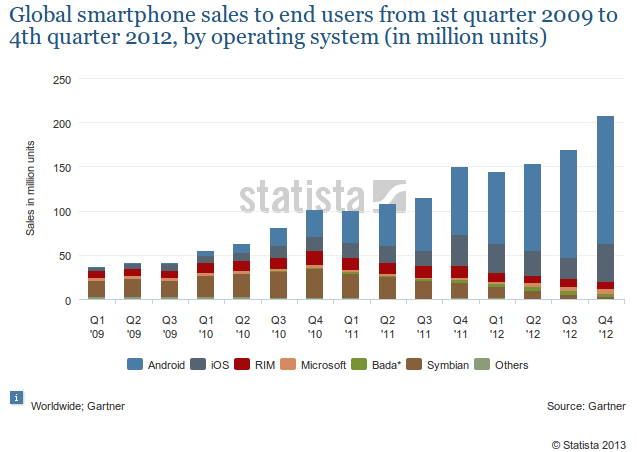
\includegraphics[scale=0.6]{images/sale}
\caption{Verkaufszahlen von Smartphones weltweit nach Plattform}
\label{sale1}
\end{figure}
\end{center}

aktueller vorreite der brache ist das auf linux basierende betriebssystem android von google. die wachsende beliebtheit dieses betriebsystems für tablets und smartphone amcht es umso interresanter für entwickler applikationen und services für geräte zu entwickeln die dieses betriebssystem nutzen.

um einen einblick in die entwicklung von applikationen für das mobile betriebsystem haen wir uns daher für die entwicklung einer applikation für die besagte platvor entschieden.

die geplante applikation soll einen vorbestimmten zweck dienen und einen nutzen erfüllen.

\subsection{Vorwort}
Die arbeit soll einblicke in die entwicklung von applikationen für das betriebsystem android gewähren. Es wernden die grundstrukturen von android vorgestellt und erläutert. diese grundstrukcturen sind äußerst wichtig um die art und weise wie applikationen auf der platform ausgeführt werden und vom nutzer verwendet werden.

abshcließend werden verschiedene probleme und lösungswege wärend den konzeptionierung und implementierung sowie der projektbearbeitung erläutert.

desweiteren werden ver\footnote{http://www.statista.com/statistics/74592/quarterly-worldwide-smartphone-sales-by-operating-system-since-2009/}schiedene schritte von konzeptionierung sowie implementierung verschiedener komponentenstrukturen der applikation diskutiert und ausgewertet. das letzendliche ziel der arbeit ist eine nutzbare zweckgerichtete applikation.


